\normalfalse \difficiletrue \tdifficilefalse
\correctionfalse

%\UPSTIidClasse{11} % 11 sup, 12 spé
%\newcommand{\UPSTIidClasse}{11}

\exer{Système EPAS  $\star\star$ \label{C2:07:64}}
\setcounter{question}{0}\UPSTIcompetence[2]{C2-07}
\index{Compétence C2-07}
\index{PFS}
\index{EPAS}
\ifcorrection
\else
\marginnote{\textbf{Pas de corrigé pour cet exercice.}}
\fi
\ifprof
\else

Le véhicule porteur de l’E.P.A.S. doit être équipé de stabilisateurs. Une fois en place, les
stabilisateurs le soulèvent, afin qu’il ne repose plus sur les roues (les roues touchent le sol mais ne
supportent aucun poids) : le mouvement des suspensions du véhicule mettrait en danger sa stabilité.

L’objet de cette partie est de déterminer la longueur de déploiement maximale que le système de
sécurité pourra autoriser.

\begin{center}
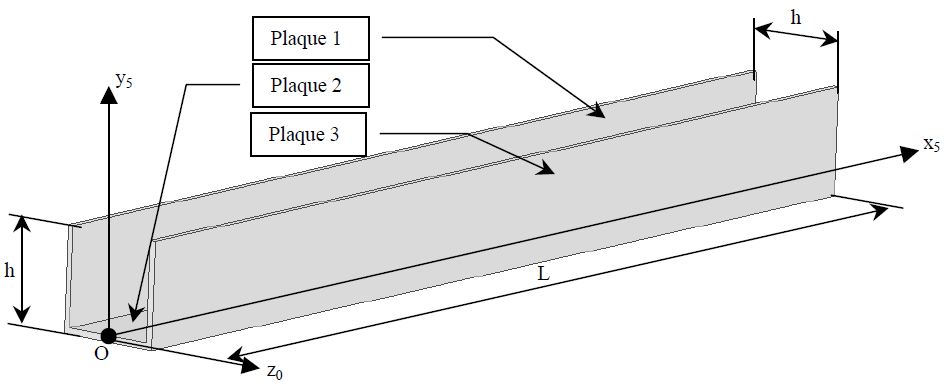
\includegraphics[width=\linewidth]{64_01}
\end{center}

Le véhicule est dans la configuration de la figure précédente :
\begin{itemize}
\item parc échelle horizontale;
\item stabilisateurs sortis au maximum;
\item charge maximale dans la plate-forme.
\end{itemize}

Le problème sera traité en statique plane dans le plan $\left(O, \vect{x}, \vect{y}\right)$ de la figure précédente.

Les efforts pris en compte sont :
\begin{itemize}
\item les actions de pesanteur sur chaque élément :
\begin{itemize}
\item véhicule et charge utile, centre d'inertie $G_V$, masse $m_V$, $\vect{OG_V}=a\vect{y}$,
\item parc échelle, centre d'inertie $G_E$, masse $m_E$, $\vect{OG_E}=\dfrac{L}{2}\vect{x}+h\vect{y}$,
\item plate-forme et charge utile, centre d'inertie $G_P$, masse $m_P$, $\vect{OG_P}={L}\vect{x}+H\vect{y}$;
\end{itemize}
\item les actions de contact de la route sur les stabilisateurs.
\end{itemize}

Ces actions sont modélisées par des glisseurs passant l'un par $M$, tel que $\vect{OM}=-b\vect{x}$ et l'autre par $N$ tel que $\vect{ON}=b\vect{x}$. 
Les résultantes de ces glisseurs seront notées respectivement : $\vect{R}_M=X_M\vect{x}+Y_M\vect{y}$ 
et $\vect{R}_N=X_N\vect{x}+Y_N\vect{y}$.

\fi

\question{Exprimer la condition de non basculement de l’ensemble.}
\ifprof
\else
\fi

\question{Calculer la longueur $L_{\text{max}}$ de déploiement au-delà de laquelle il y aura basculement.}
\ifprof
\else
\fi


\ifprof
\footnotesize
\begin{enumerate}
\item .
\item $L_{\text{max}}=2b\dfrac{m_P+m_E+m_V}{2m_P+m_E}$.
\end{enumerate}
\normalsize
\else
\begin{flushright}
\footnotesize{Corrigé  voir \ref{C2:07:64}.}
\end{flushright}%
\fi